\section{对偶块复形}
\sourcepage{455--456}
为简便起见，接下来几节先只讨论同调 $n$ 维流形 $X$。所用方法以后还将在相对同调流形的情形中出现。

对于已三角剖分的同调流形，可以把 $X$ 分成一些“几乎”是开胞腔的子集，使其“几乎”成为正则胞腔复形。这些子集不是实际的拓扑胞腔，而只是同调意义的胞腔，因此称它们为\emph{块}，并称所得分解为 $X$ 的\emph{对偶块分解}。与胞腔复形一样，块复形也有一个可用于计算 $X$ 同调和上同调的链复形，称为\emph{对偶链复形}。这是证明对偶定理的关键工具。

回顾第 2.3 节，$\sigma_1\succ\sigma_2$ 表示 $\sigma_2$ 是 $\sigma_1$ 的真面。

\entry{定义}{8.4.1}设 $X$ 是局部有限单纯复形，$\operatorname{sd}X$ 为第一次重心重分。由引理 2.3.9，其单形形如
\[
\widehat\sigma_{i_1}\widehat\sigma_{i_2}\cdots\widehat\sigma_{i_k},
\qquad\sigma_{i_1}\succ\sigma_{i_2}\succ\cdots\succ\sigma_{i_k}.
\]
始终按此顺序排列顶点。为便于记录，称第一个顶点为该单形的\emph{最大顶点}，最后一个为\emph{最小顶点}。

\entry{例}{8.4.2}设 $X$ 是平面中顶点为 $a,b,c$ 的三角区域，视为二维单纯复形。其重心重分的顶点为
\[a,b,c,\quad\widehat{ab},\widehat{bc},\widehat{ca},\quad\widehat{abc}.\]
顶点 $\widehat{abc}$ 在任何包含它的单形中都是最大顶点；以它为最小顶点的单形只有它自身。$\widehat{ab}$ 是边 $\widehat{ab}a,\widehat{ab}b$ 以及零维单形 $\widehat{ab}$ 的最大顶点，也是边 $\widehat{abc}\widehat{ab}$ 以及它自身的最小顶点。

\entry{定义}{8.4.3}给定 $X$ 的单形 $\sigma$，注意以 $\widehat\sigma$ 为最大顶点的所有重分后开单形的并恰为 $\Int\sigma$。另一方面，定义 $D(\sigma)$ 为以 $\widehat\sigma$ 为最小顶点的所有开单形之并，称为\emph{与 $\sigma$ 对偶的块}。

这些块起到类似 CW 复形开胞腔的作用。其闭包 $\overline D(\sigma)$ 称为\emph{对偶闭块}，是所有末顶点为 $\widehat\sigma$ 的单形及其面的并，因而是 $\operatorname{sd}X$ 的子复形的多面体。记
\[\dot D(\sigma)=\overline D(\sigma)\setminus D(\sigma).\]

\begin{figure}[htbp]\centering
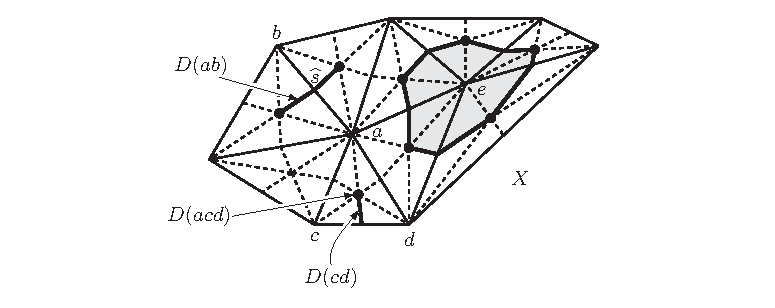
\includegraphics[width=.88\textwidth]{figures/8-4-1.pdf}
\caption*{图 8.4.1}
\end{figure}

\entry{例}{8.4.4}设 $X$ 为图 8.4.1 的二维复形，虚线表示其重心重分。每个二维单形的对偶块只有其重心。边 $s=ab$ 的对偶块由重心 $\widehat s$，以及从它连接到以该边为面的两个三角形重心的两条开线段组成。顶点 $e$ 的对偶块是图中的阴影区域，相应闭块还包括该区域边界。值得注意的是，$\dot D(e)$ 是所有以 $e$ 为面的边和三角形所对应的低维对偶块之并。我们很快就会证明这普遍成立。

\sourcepage{457}
\entry{例}{8.4.5}图 8.4.2 的复形是四边形 $cdefc$ 与线段 $ab$ 的联结。读者可以想象其重心重分。每个三维单形的对偶块是其重心。三角形 $abc$ 的对偶闭块由两条线段组成，连接该三角形重心与以它为面的两个三维单形的重心。边 $ab$ 的对偶闭块是图 8.4.3 的闭八边形区域；$\dot D(ab)$ 为其边界，是所有以 $ab$ 为面的二维、三维单形的对偶块之并。

\begin{figure}[htbp]\centering
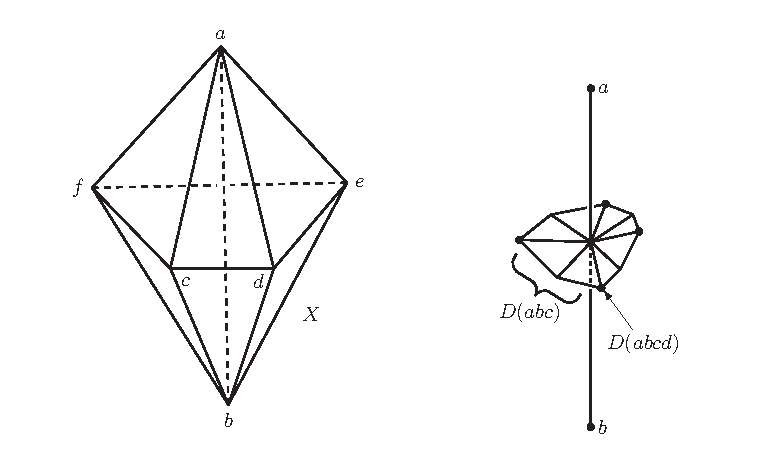
\includegraphics[width=.96\textwidth]{figures/8-4-2-3.pdf}
\caption*{图 8.4.2（左）与图 8.4.3（右）}
\end{figure}

证明下一定理时，请记住这两个例子。

\entry{定理}{8.4.6}设 $X$ 是局部有限单纯复形，完全由 $n$ 维单形及其面组成，$\sigma$ 是其中一个 $k$ 维单形。则：
\begin{enumerate}[label=(\alph*)]
\item 各对偶块不交，其并为 $|X|$。
\item $\overline D(\sigma)$ 是 $\operatorname{sd}X$ 的一个 $(n-k)$ 维子复形的多面体。
\item $\dot D(\sigma)$ 是所有满足 $\tau\succ\sigma$ 的块 $D(\tau)$ 的并；这些块的维数均小于 $n-k$。
\item $\overline D(\sigma)=|\dot D(\sigma)*\widehat\sigma|$。
\item 若 $\widehat\sigma$ 处局部同调只在 $n$ 维为 $\Z$，则 $(\overline D(\sigma),\dot D(\sigma))$ 具有 $(n-k)$ 维胞腔模其边界的同调。
\end{enumerate}

\textbf{证明：}(a) 重分后的开单形两两不交，每个恰位于一个块中，即其最小顶点所对应的块。

\sourcepage{458}
(b) 取以 $\sigma$ 为面的 $n$ 维单形 $\sigma'$，可以找到逐次降低一维的面链
\[\sigma'=\sigma_n\succ\sigma_{n-1}\succ\cdots\succ\sigma_k=\sigma.\]
由这些重心组成的重分后单形维数为 $n-k$，且位于 $\overline D(\sigma)$ 中。由于 $X$ 没有高于 $n$ 维的单形，以 $\widehat\sigma$ 为末顶点的单形不可能有更高维数。

(c)、(d) 闭块由所有形如
\[\widehat\sigma_{i_1}\cdots\widehat\sigma_{i_p}\widehat\sigma\]
的单形及其面组成。这样的单形与 $\dot D(\sigma)$ 的交，是删去末顶点所得的面。因此 $\dot D(\sigma)$ 由所有满足 $\sigma_{i_p}\succ\sigma$ 的单形 $\widehat\sigma_{i_1}\cdots\widehat\sigma_{i_p}$ 组成，其内部恰位于 $D(\sigma_{i_p})$ 中。反之，这些块中的每个开单形都有此形式。于是得到 (c)，同时也得到锥的描述 (d)。

(e) 若 $k=n$，闭块只有重心，是零维胞腔。设 $k<n$。在重分复形中，$\widehat\sigma$ 的闭星形邻域由顶点面链中包含 $\sigma$ 的所有单形组成。在面链中位于 $\sigma$ 之前的部分组成 $\dot D(\sigma)$ 的单形，$\sigma$ 及其后的部分组成 $\operatorname{sd}\sigma$ 的单形。因此
\[
\overline{\operatorname{St}}(\widehat\sigma,\operatorname{sd}X)
=\dot D(\sigma)*\operatorname{sd}\sigma
=\dot D(\sigma)*\widehat\sigma*\operatorname{sd}(\Bd\sigma).
\]
另一方面，闭星形邻域等于 $\widehat\sigma*\operatorname{Lk}(\widehat\sigma,\operatorname{sd}X)$，所以
\[\operatorname{Lk}(\widehat\sigma,\operatorname{sd}X)=\dot D(\sigma)*\operatorname{sd}(\Bd\sigma).\]
由于 $\operatorname{sd}(\Bd\sigma)$ 是拓扑 $(k-1)$ 维球面（$k=0$ 时为空），
\[\widetilde H_{i+k}(\operatorname{Lk}(\widehat\sigma,\operatorname{sd}X))\cong\widetilde H_i(\dot D(\sigma)).\]
\sourcepage{459}
由局部同调假设及引理 8.3.2，左侧链环是同调 $(n-1)$ 维球面，故 $\dot D(\sigma)$ 是同调 $(n-k-1)$ 维球面。闭块为锥，故无环，其同调长正合列给出
\[H_i(\overline D(\sigma),\dot D(\sigma))\cong\widetilde H_{i-1}(\dot D(\sigma)),\]
于是得到胞腔模边界的同调。\hfill$\square$

\entry{定义}{8.4.7}设 $X$ 是局部有限的同调 $n$ 维流形复形。\footnote{事实上，每个作为同调 $n$ 维流形的复形都是局部有限的。}上一定理适用于每个单形。所有对偶块组成 $X$ 的\emph{对偶块分解}。维数不超过 $p$ 的块之并记作 $X_p$，称为\emph{对偶 $p$ 维骨架}。定义\emph{对偶链复形} $\mathcal D(X)$：
\[\mathcal D_p(X)=H_p(X_p,X_{p-1}),\]
边缘算子为三元组 $(X_p,X_{p-1},X_{p-2})$ 的正合列中的连接同态 $\partial_*$。

对偶骨架是 $\operatorname{sd}X$ 的子复形的多面体，因而有时把它直接视为复形。特别地，为方便起见，定义 $\mathcal D_p(X)$ 时采用单纯同调。

对偶链复形在计算同调和上同调中的作用，实际上与 CW 复形的胞腔链复形相同。仿照第 4.13 节，得到如下结论。

\entry{定理}{8.4.8}设 $X$ 是局部有限的同调 $n$ 维流形复形，$X_p$ 为对偶骨架。
\begin{enumerate}[label=(\alph*)]
\item $H_i(X_p,X_{p-1})$ 在 $i\ne p$ 时为零，$i=p$ 时为自由阿贝尔群。一组基可以如下取得：对每个 $p$ 维块，选取 $H_p(\overline D(\sigma),\dot D(\sigma))$ 的生成元，再取其在包含映射诱导的同态下的像。
\item $\mathcal D(X)$ 可用于计算 $X$ 的同调。确切地说，$\mathcal D_p(X)$ 可等同于 $C_p(\operatorname{sd}X)$ 中承载于 $X_p$ 且边界承载于 $X_{p-1}$ 的链所组成的子群。包含映射诱导同调同构，因而也诱导任意系数的同调和上同调同构。\translatornote{原文这句把链的承载空间写为 $X$；按定义应为对偶骨架 $X_p$。}
\end{enumerate}

\sourcepage{460}
\textbf{证明：}(a) 仿照引理 4.13.4，但更为简单。每个闭块是以 $\widehat\sigma$ 为顶点的锥，删去顶点后可形变收缩到 $\dot D(\sigma)$。这些形变收缩合起来，给出
\[X_p\setminus\bigcup_p\{\widehat\sigma\}\longrightarrow X_{p-1}\]
的形变收缩，其中并集遍历所有 $(n-p)$ 维单形的重心。考虑所有 $p$ 维闭块偶的拓扑和。先把每个偶 $(\overline D(\sigma),\dot D(\sigma))$ 的第二项扩大为删去重心的闭块；由形变收缩，诱导同调同构。将拓扑和映入 $(X_p,X_p\setminus\bigcup_p\{\widehat\sigma\})$，再由切除得到各局部部分的同调直和。对应的包含映射给出交换图，并得到
\[
\bigoplus_{\dim D(\sigma)=p}H_i(\overline D(\sigma),\dot D(\sigma))
\cong H_i(X_p,X_{p-1}).
\]
于是 (a) 对奇异同调成立，因而也对单纯同调成立。(b) 直接由定理 4.13.9 得到。\hfill$\square$

我们现已具备证明 Poincaré 对偶定理的基本工具。

\sourcepage{460--461}
\subsection*{习题}
\begin{enumerate}
\item 考虑环面 $T$ 的通常三角剖分。
\begin{enumerate}[label=(\alph*)]
\item 画出对偶块分解。注意这些块实际上使 $T$ 成为正则胞腔复形。
\item 设 $C(T)$ 为单纯链复形，$\mathcal D(T)$ 为对偶链复形。把二维单形逆时针定向，边任意定向。对每个有向二维单形，令
\[\varphi:C^2(T)\to\mathcal D_0(T),\qquad\varphi(\sigma^*)=D(\sigma)=\widehat\sigma.\]
再定义同构 $\varphi:C^1(T)\to\mathcal D_1(T)$，使 $\varphi(e^*)$ 为 $(\overline D(e),\dot D(e))$ 的一个基本闭链。证明可以选择这些基本闭链，使 $\partial\varphi(e^*)=\varphi(\delta e^*)$。
\item 定义 $\varphi:C^0(T)\to\mathcal D_2(T)$，使 $\varphi(v^*)$ 为 $(\overline D(v),\dot D(v))$ 的基本闭链。证明若二维胞腔 $D(v)$ 逆时针定向，则 $\partial\varphi(v^*)=\varphi(\delta v^*)$。
\item 得出对所有 $p$ 都有 $H^p(T)\cong H_{2-p}(T)$（这一点我们已经知道）。
\end{enumerate}
这道习题展示了 Poincaré 对偶的证明方法。
\item 对 Klein 瓶重复习题 1，同调和上同调都取 $\Z/2$ 系数。注意不涉及符号，所以证明更容易。
\item 若把前两题中的环面和 Klein 瓶换成球面，可以得到什么结论？
\item 若把前两题中的对象换成双环面（有两个孔），可以得到什么结论？
\end{enumerate}
